%
\documentclass[conference]{IEEEtran}
\ifCLASSINFOpdf

\else \fi

\hyphenation{op-tical net-works semi-conduc-tor}

\usepackage[square, comma, sort&compress, numbers]{natbib}
\usepackage{graphicx}
\usepackage{subfigure}
\usepackage{caption}
\usepackage{mathrsfs}
\usepackage{algorithm}
\usepackage{algpseudocode}
\usepackage{amsthm}
\usepackage{amsmath}
\usepackage{graphics}
\usepackage{epsfig}
\usepackage{amssymb}
\usepackage{multirow}
\usepackage{setspace}
\usepackage[table]{xcolor}
\usepackage{breqn}
\usepackage{url}
\usepackage{caption}
\usepackage{color,colortbl}
\usepackage{xspace}
\usepackage{booktabs}


\newtheorem{assump}{Assumption}
\newtheorem{axiom}{Axiom}
\newtheorem{claim}{Claim}
\newtheorem{conj}{Conjecture}[section]
\newtheorem{crit}{Criterion}
\newtheorem{theorem}{Theorem}
\newtheorem{coro}{Corollary}[theorem]
\newtheorem{definition}{Definition}
\newtheorem{example}{Example}
\newtheorem{fact}{Fact}
\newtheorem{hypo}{Hypothesis}
\newtheorem{lemma}{Lemma}
\newtheorem{obsv}{Observation}[theorem]
\newtheorem{prin}{Principle}
\newtheorem{prob}{Problem}
\newtheorem{ppty}{Property}
\newtheorem{propo}{Proposition}
\newtheorem{protocol}{Protocol}
\newtheorem{remark}{Remark}
\newtheorem{test}{Test}
\newtheorem{transform}{Conversion Algorithm}

\newcommand{\tabincell}[2]{\begin{tabular}{@{}#1@{}}#2\end{tabular}}
\renewcommand\d{\mathop{}\!\mathrm{d}}
\newcommand{\systemname}{WiMi\xspace}

\newcommand{\CSI}{\texttt{CSI}\xspace}
\newcommand{\RSSI}{\texttt{RSSI}\xspace}
\newcommand{\RF}{\texttt{RF}\xspace}
\newcommand{\UWB}{\texttt{UWB}\xspace}
\newcommand{\FMCW}{\texttt{FMCW}\xspace}
\newcommand{\RFID}{\texttt{FMCW}\xspace}
\newcommand{\AoA}{\texttt{AoA}\xspace}
\newcommand{\TOF}{\texttt{TOF}\xspace}
\newcommand{\OFDM}{\texttt{OFDM}\xspace}

\definecolor{Gray}{gray}{0.9}

\newcommand\FIXME[1]{\textcolor{orange}{FIX:}\textcolor{orange}{#1}}
\newcommand\red[1]{\textcolor{red}{\textcolor{red}{#1}}}


\begin{document}

%
\title{Sensing Our World Using Wireless Signals}


\author{}

\maketitle

\begin{abstract}
In the last decades, consumer-grade wireless signals have rapidly established as a powerful medium for sensing. By measuring how the
wireless signal is affected by objects and human activities, rich information ranging from gestures to gait patterns and even vital
 signs can be identified. This article provides an accessible introduction to wireless sensing. It presents the key enabling technology of
this exciting research field and its main achievements. It provides a discussion on open issues in the area and potential research
directions.
\end{abstract}


\IEEEpeerreviewmaketitle

\section{Introduction}
%Wireless signals, such as WiFi and the radio frequency (\RF), have emerged as a cheap yet powerful medium for information sensing. By
%measuring how the wireless signal is affected by surrounding objects and human activities, tasks like gait identification~\cite{}, gesture
%recognition~\cite{}, activity recognition~\cite{}, and vital sign monitoring~\cite{} can be possible.
%
%
%The desire for employing wireless signals for sensing could date back to the 19th century  for the discovery of X-rays for object
%recognition~\cite{} and the development of military radar and sonar systems for tracking large metallic objects in open
%spaces~\cite{Charles Samuel Franklin 's development of first practcial radar}. These sensing systems, however, have to rely on expensive specialize hardware and be operated by professionals, which thus put they out of the reach of ordinary people.
%
%
%Recently, it has been shown that wireless sensing built upon consumer-grade devices such as smartphones and wireless routers can be used to
%precisely track human activities in an indoor environment. Such technology has the advantages of being low-cost as it requires as few as
%two wireless routers to operate, not requiring instrumenting the user, being less privacy intrusive compared to other infrastructure-based
%solutions like video-based solutions~\cite{}, and is safer to use on a regular basis compared to other alternatives like X-rays~\cite{}. It
%offers an inexpensive way for bringing activity sensing into everyday life -- which not only makes ever sensing a tantalizing reality but
%could also open up new possibilities for innovative applications.
%
%
%As we will show in this article, while there are still many challenges ahead, consumer-grade wireless sensing has moved from a research
%niche to a mainstream activity. This is, in fact, a dynamic field looking at subjects as diverse as smart-home personalization~\cite{} and
%fall monitoring~\cite{} to emotion detection~\cite{}. In this article we aim to demystify this promising technique, outline the challenges
%it is facing, and show that this is a trustworthy and exciting research direction.
%
%
%
%
%The remainder of this article is structured as follows. We first give an intuitive view for the wireless sensing working mechanism  in
%Section~\ref{sec:mechanism}. \FIXME{We then describe xx, bla bla...}. We discuss the challenges and limitations for wireless sensings, as
%well as open research directions in Section xx before we summarise and conclude in Section \FIXME{xx}.

Wireless signals, such as WiFi and the radio frequency (\RF), have emerged as a cheap yet powerful medium for information sensing. By
measuring how the wireless signal is affected by surrounding objects and human activities, tasks like localization~\cite{Arraytrack,
Tagoram}, activity recognition~\cite{Wang2015Understanding, wang2016human}, and material identification~\cite{Tagscan, LiquID, zhao2018rf}
could be possible.


The history for using wireless signals for sensing dates back to the 19th century  for the discovery of X-rays for object
recognition~\cite{Suzuki1996} and the development of military radar and sonar systems for tracking large metallic objects in open
spaces~\cite{}. These sensing systems, however, have to rely on expensive specialize hardware and be operated by professionals, which thus
put they out of the reach of ordinary people.


Recently, it has been shown that wireless sensing built upon consumer-grade devices such as smartphones and wireless routers can be used to
precisely track objects and human activities in an indoor environment. Such technology has the advantages of being low-cost as it requires
as few as two wireless routers to operate, not requiring instrumenting the user, being less privacy intrusive compared to other
infrastructure-based solutions like video-based solutions~\cite{Cruz2015Quantification}, and is safer to use on a regular basis compared to
other alternatives like X-rays~\cite{De2013B}. It offers an inexpensive way for bringing the sensing capability into everyday life, making
ever sensing a tantalizing reality.

As we will show in this article, while there are still many challenges ahead, consumer-grade wireless sensing has moved from a research
niche to a mainstream activity. This is, in fact, a dynamic field looking at subjects as diverse as smart-home personalization~\cite{} and
fall monitoring~\cite{} to emotion detection~\cite{} and vital sign monitoring~\cite{}. In this article we aim to demystify this promising
technique, outline the challenges it is facing, and show that this is a trustworthy and exciting research direction.




%The remainder of this article is structured as follows. We first give an intuitive view for the wireless sensing working mechanism  in
%Section~\ref{sec:mechanism}. \FIXME{We then describe xx, bla bla...}. We discuss the challenges and limitations for wireless sensings, as
%well as open research directions in Section xx before we summarise and conclude in Section \FIXME{xx}.


%
%The development of wireless devices has resulted in numerous wireless sensing technologies which enable a variety of applications such as
%indoor navigation, smart homes, fitness tracking and security check. In recent years, especially non-contact wireless sensing has attracted
%much attention from both the research community and the industry, due to its convenience of without instrumenting user's body. Many
%researches have answered how to identify object's location, shape, material, behavior, etc. The basic idea of these designs is to utilize
%signal processing to construct a mapping pattern or theoretical relationship between the target information and the signal characteristics.
%
%To turn these designs into practical systems, series challenges need to be tackled. Typically, (i) the defects of cheap devices can lead to
%nonnegligible error of signal information~(phase), (ii) environmental changes can alter the regular signal patterns, and (iii) multi-path
%effect would greatly reduce the estimation resolution of some fundamental parameters for sensing. These always make the system performance
%extremely poor. To address these issues, many efforts has been made, including: (i) calibrating the inaccurate phase information through
%comparing with it with a real value obtained in advance, (ii) canceling background noise using signals from multiple links, and (iii)
%improving the resolution of parameter estimation by splicing bandwidth or constructing virtual array. Nowadays, with the popularity of
%artificial intelligence, deep learning technology is gradually integrated into signal processing to extract more complex and effective
%features for sensing task. This drives great success in wireless sensing applications.
%
%In the rest of this paper, we first review the state-of-arts of wireless sensing. Then we conclude the key challenges of this field and
%suggest promising solutions for them. Finally, we propose guiding insights into future trends.

\section{How Does It Work?\label{sec:mechanism}}
\begin{figure} [t!]
       \centering
        \subfigure[]{
                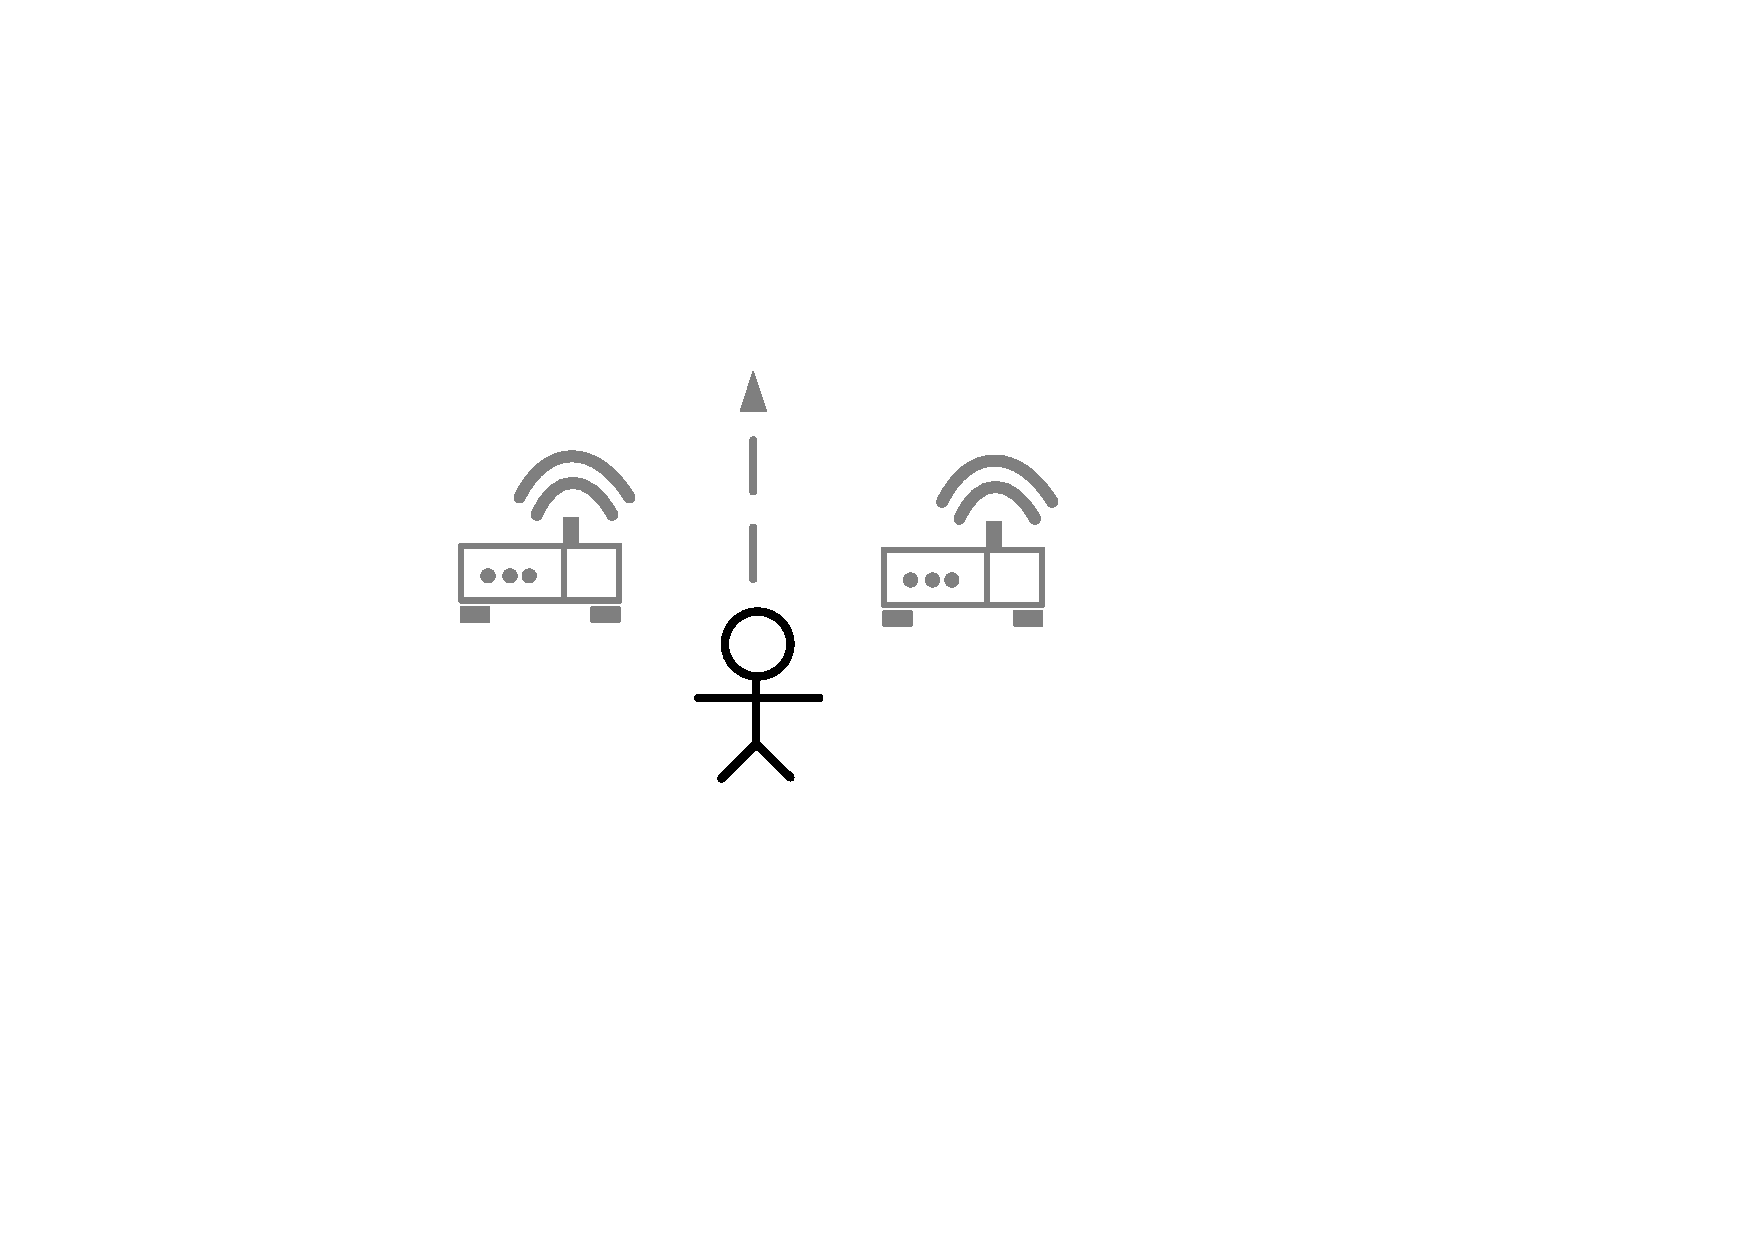
\includegraphics[width=0.22\textwidth]{figures/setup_example.pdf}
                \label{fig:scenario_1}
        }
        \subfigure[]{
                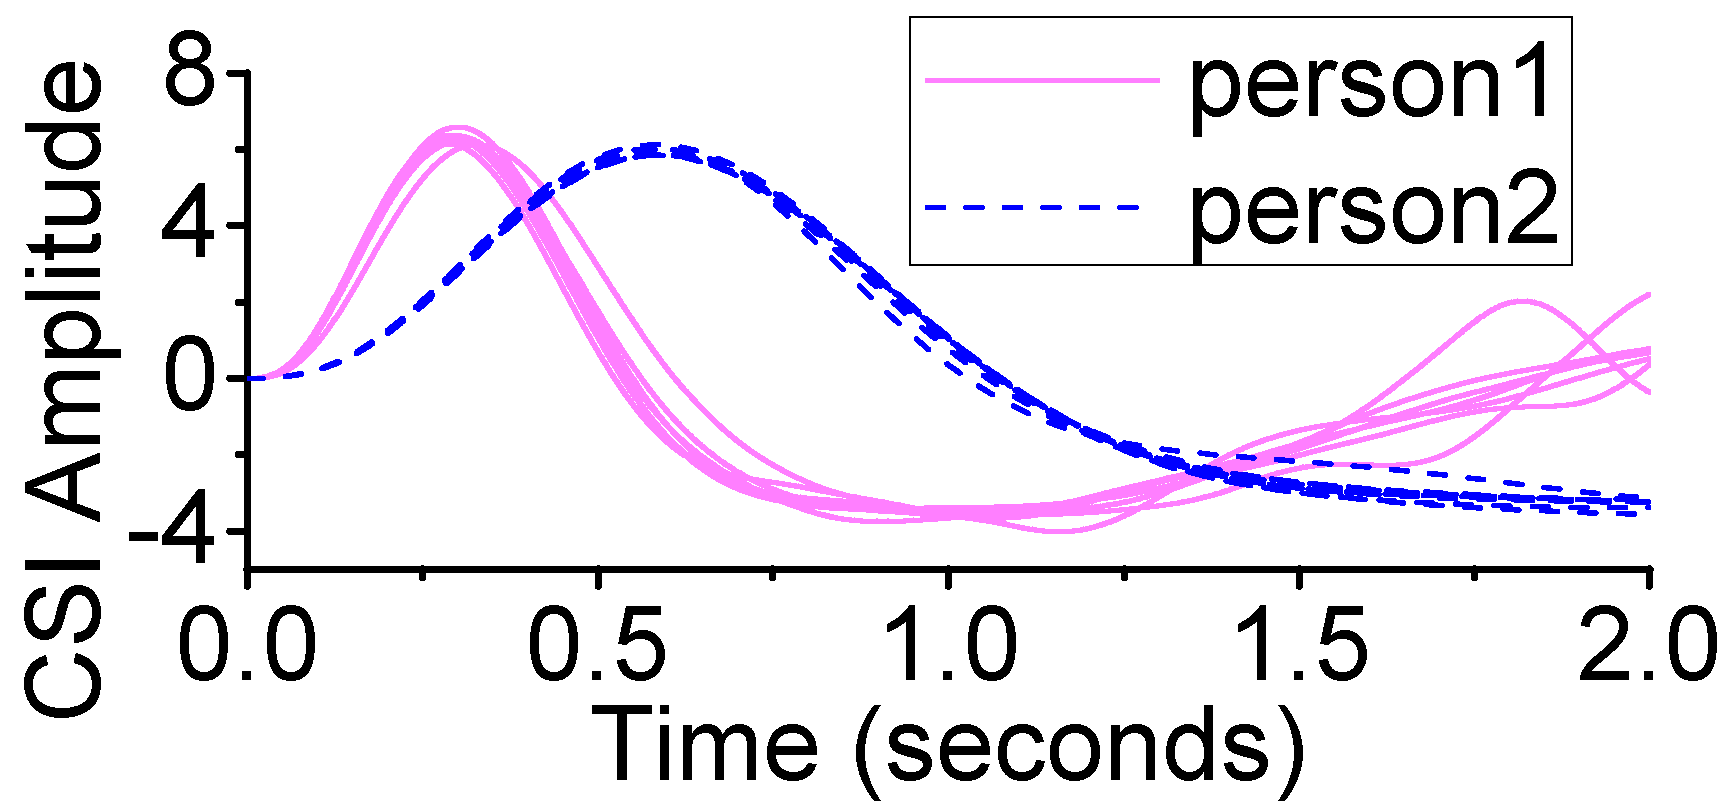
\includegraphics[width=0.22\textwidth]{figures//diff.pdf}
                \label{fig:csi_diff}
        }%
     \caption{The working mechanism of wirless sensing. (a) shows a typical set up where two wireless devices are deployed
     to collect the \CSI values when a user walks pass the devices. (b)  shows the measured \CSI  for two
     individuals, where the resulted \CSI amplitudes are relatively consistent for the same person across multiple walks, but are sufficiently different for different people.}
     \label{fig:csi_demo}
\end{figure}


To illustrate the working mechanism of wireless sensing, consider the gait identification scenario depicted in Figure~\ref{fig:scenario_1}.
The sensing task in this example is to identify which of a set of known users has walked pass the scene. Knowing this information allows
one to -- for example -- personalize the light setting of a smart home. Here, two wireless routers (a sender and a receiver) are used to
measure how the user's movement affect the wireless channel metric, such as the channel state information (\CSI) or received signal
strength indicator (\RSSI). The idea is that the wireless signal will bounce off the wall, furniture, and human body, and the unique
behavior of a person's activity (walking in this example) would lead to a unique pattern in the wireless signal; by measuring how the
wireless signal is affected by the human activity and comparing the measurement against some pre-collected fingerprints or training data,
one can infer what activity has been performed and by whom.

Figure~\ref{fig:csi_diff} shows the measured \CSI amplitudes of two users in our scenario. In this case, each user walked through our scene
five times and the \CSI amplitude per walk is shown. This figure suggests that wireless channel metrics can be a useful means for user
identification, because the channel metric measurements for the same person is relatively consistent but is sufficiently different for the
two  people.

Note that although the setup and the sensing method would vary depending on the sensing task and the wireless signal to use, this example
shares many of the commonalities of wireless sensing, which demonstrates the underlying working principal of wireless sensing.

\subsection {Choices of Wireless Sensing Signals}

\renewcommand\arraystretch{2}
\begin{table*}\scriptsize
%\centering
\caption{Consumer-grade wireless signals used in prior sensing tasks.}
\label{Tab1}
\setlength{\tabcolsep}{7mm}
\begin{tabular}{p{1cm}p{0.6cm}<{\raggedright}p{0.9cm}<{\raggedright}p{0.7cm}<{\raggedright}p{0.6cm}<{\raggedright}p{1.1cm}<{\raggedright}p{0.8cm}<{\raggedright}p{1.2cm}<{\raggedright}}
\toprule
%\diagbox[width=5em,trim=l]{Properties}{Signal} & Wi-Fi & RFID & UWB & Asoustic & LoRa & FMCW radar & Visible Light \\
\textbf{Properties} & \textbf{WiFi} & \textbf{RFID} & \textbf{UWB} & \textbf{Asoustic} & \textbf{LoRa} & \textbf{FMCW radar} & \textbf{Visible Light} \\
\midrule
\rowcolor{Gray} \textbf{Communication Range} & 35m & 10m & 10-20m & 2-3m & 15km & 9m-120km & 1.4km\\
\textbf{Frequency} & 2.4GHz/5GHz & 902.75-927.25MHz & 3.1-10.6GHz & 17-24KHz & 868MHz/903-927.5MHz & 24-24.25GHz & 380-790THz\\
\rowcolor{Gray} \textbf{Bandwidth} & 20/40MHz & 24.5MHz & 1GHZ & -- & 125/250/500KHz & 250MHz & --\\
\textbf{Metrics} & CSI, \RSSI & Phase, Doppler, \RSSI & Phase, \RSSI& Phase, \RSSI & Frequency, Phase, \RSSI & Frequency, Phase, \RSSI & \RSSI\\
\rowcolor{Gray} \textbf{Cost} & Low & Low & High & Low & Low & High & High\\
%\textbf{Modulation} & OFDM & OOK & PPM & AM/FM/PM & CSS& FMCW & OOK/CSK/VPPM\\
\bottomrule
\end{tabular}
%\caption{Different wireless signals with different properties.}%\lable{Tab1}
\end{table*}

As summarized in Table~\ref{Tab1}, a wide range of wireless signals have been employed in prior work for information sensing. These include
\WiFi, \RFID, acoustic, long-range (\LoRa) signal, visible lights, frequency-modulated continuous-wave (\FMCW) radar and ultra-wideband (\UWB). Signals like
WiFi, acoustic, and visible lights are readily available on commercial off-the-self devices (such as smartphones and smart light bulbs),
while others like \UWB and \FMCW often require specialize hardware to operate.



Which signal is best for a sensing task, is the \$64,000 question. The answer is, it depends. For examples, while \WiFi is almost
everywhere, it is limited in the communication range (i.e., 35 meters) and consumes a significant amount of power; by contrast, \LoRa
supports a longer range (i.e., 15 Kilometers) and needs significantly less power to operate, but it has a much lower bandwidth and is more
sensitive to the environmental multipath. Different signals also operate at different frequencies and offer a variety of sensing metrics.
Some of the signals like \FMCW radar can provide an accurate tracking capability but is more expensive to deploy. It is important to note
that there is no ``one-size-fits-all" sensing medium, and the choice depends on the trade-off between the precision requirements, the
deployment environment, and the budget.

\section {Various sensing applications}

In recent years, with the emerging of the Internet of Thing (IoT), many wireless sensing applications have been inspired, especially for
localization and tracking, behavior perception, material identification, target imaging and vibration detection. In this section, we will
present these five mainstream applications respectively. We also discuss the challenges coming with them and corresponding efforts have
made.

\subsection{Localization and Tracking} Target localization and tracking are two most universal and significant sensing applications.
Specifically, indoor localization has attracted much interest from both the industry and the research community. Among all the technologies
employed for localization, Wi-Fi and RFID are considered as the most promising schemes due to the cheap price and widespread deployment.
Furthermore, we can easily access the amplitude and phase information from commercial RFID and Wi-Fi devices. In the following, we will
discuss previous indoor localization works, which can be classified into two categories: learning-based and model-based localization
schemes.

\textbf{Learning-based localization:} These systems collect received signal strength~(RSS) and channel state information~(CSI) at each
location to build fingerprints for localization, which can achieve a meter-level accuracy. Although these systems are easy to be deployed,
their localization accuracies are susceptible to environmental change and indoor multi-path. Furthermore, learning-based localization
schemes suffer from labor-intensive offline training.

\textbf{Model-based localization:} For a robust, higher accuracy and low cost system, more and more researches have a trend to explore
model-based localization approaches, which can be divided into two categories. The first category of localization systems are based on
arrival-of-angle~(AoA) or time-of-flight~(TOF) estimation, which achieve localization by intersecting multiple AoA or ToF estimates. The
second category is energy-attenuation-based localization systems, which establish signal energy attenuation model to calculate target
localization. These ideas sound simple, however, there exist some common challenges to make them practical.

\paragraph*{Hardware imperfections} Due to commercial hardware imperfections, we cannot obtain accurate phase information and accurate time of
flight.

\paragraph*{multi-path effect} In our indoor environment, there exits rich  multi-path effects, which result in the inaccuracy of location
parameter estimation and signal attenuation model construction.

\paragraph*{Uncertainty of initial position} For the tracking systems, it is difficult to determine target's initial position.



 To mitigate the phase error caused by commercial hardware imperfections, a general idea is to calibrate phase information by comparing it
 with the real pre sampled values \cite{Wang2016D}. Meanwhile, different frequencies can be utilized to emulate a very large bandwidth for
 achieving accurate time estimation~\cite{RFind}. To eliminate the multi-path effect, on the one hand, we can conversely exploit multi-path
 to capture multi-path profiles for target localization~\cite{PinIt}. On the other hand, by increasing the number of antennas in the array,
 we can improve angle estimation resolution to identify the line-of-sight~(LoS)~\cite{Arraytrack, Spotfi}. Furthermore, one skillful idea
 is to select clear subcarrier information to establish signal attenuation model~\cite{wang2016lifs}. To deal with the uncertainty of
 initial position, we can leverage virtual antenna array and approximate evaluation method to improve tracking accuracy~\cite{Tagoram}.

In addition, acoustic signal has been widely used for localization and tracking, due to its slow propagation velocity and robustness to
environment changes. However, there also exist several challenges that are similar to Wi-Fi and RFID based localization systems.

The first issue need to be tackled is the inaccuracy phase information and unsynchronized time induced by the defects of commercial
acoustic devices. A standard solution is to use phase difference for tracking target location~\cite{LLAP}, another approach is employing
multiple device to avoid the time asynchrony~\cite{BeepBeep}.  The second issue is the indoor multi-path, which results in inaccuracy of
model parameters estimation. To deal with this problem, a typical intuition is to design different modulation for acoustic signal, such as
frequency modulated carrier wave~(FMCW) and orthogonal frequency division multiplexing~(OFDM) \cite{CAT,STRATA}.

\subsection{Behavior sensing} Human behavior recognition can enable a wide variety of applications, such as heath care, fitness tracking and sleep monitoring. Similarly to localization and tracking systems, human behavior recognition interfaces can also be classified as learning-based and model-based behavior recognition two categories.

\textbf{Learning-based behavior recognition:} For most irregular behaviors recognition, researches depend on pattern learning (DTW~\cite{Wang2014We}, KNN~\cite{Forster2011Incremental}, etc) to deal with it. To ensure the recognition accuracy of systems, we need to answer following questions.

The first question is how to design a high-quality feature to achieve cross-site and large-scale sensing? To answer this, a intuitive idea is performing ensemble learning to extract the unique feature of each target~\cite{CrossSense}. The other question is how to effectively label substantial data? To address this, recent work proposes to borrow vision signal to help achieve labeling task in wireless sensing ~\cite{zhao2018rf}.

\textbf{Model-based behavior recognition:} These model-based behavior recognition schemes can only be applied to analyze few human behaviors with a specific frequency range, such as coarse movements--walking, jogging, running~\cite{Wang2015Understanding} and fine-grained breathing and heart beat~\cite{Smart-homes}. These activities can be sensed according to that they can cause signal fluctuates with specific frequencies. However, the common challenge is how to eliminate the interference from the other body parts' activities? To address this, a general idea is to filter out the undesired activities beyond the target signal frequency range in frequency domain.

\subsection{Material identification} Target material identification is a key role in our life, many applications would benefit from it, such as detecting concealed weapons and determining food deterioration. Existing material identification systems such as Radar, X-Ray, CT, MRI and B-scan ultrasonography use special hardware with high frequency, large bandwidth and antenna arrays, which are extremely expensive and usually large in size. Hence, there exits some challenges to identify target material with commodity device.

How to eliminate the impact of target's size? How to remove the impact of containers and liquid reflections?

To solve the first challenge, we can design a feature, which only depends on the material type and independent of target size, such as the ratio of RSS change and phase change \cite{Tagscan}. Consider that the liquid containers and liquid reflections have some impacts on the above feature, \cite{LiquID} employs UWB devices with high bandwidth to accurate estimate the time of signal propagation, and use it to remove the impact of containers and liquid reflections.


\subsection{Target imaging and 3D reconstruction} Wireless signal can reflect off or penetrate through various objects in the environment. Thus researches attempt to utilize this to achieve object imaging.

\textbf{Reflection-based imaging:} Due to the physics of radio reflections, at any point in time, the sensor captures signal reflection from only a subset of the human body parts. \cite{Adib2017Capturing} identifies human body parts from RF snapshots across time to capture the human figure, as the consecutive RF snapshots can expose different body parts and diverse perspectives of the same body part; However, imaging results are highly sensitive to phase accuracy. Thus~\cite{Zhu2015Reusing}  proposes a new 60Ghz imaging algorithm, which images an object using only RSS recorded along the device��s trajectory, as the RSS measurements of 60Ghz are highly robust against noises in device position and trajectory tracking.~\cite{mao2018aim} proposes a new Phase Gradient Algorithm called MPGA to remove the impact of hand jitters, compensate phase errors, MPGA can effectively support acoustic imaging in a mobile context.

Occlusion is a fundamental problem in human pose estimation. Thus, \cite{Zhao_2018_CVPR}  presents a different approach that extracts pose information from the visual stream, and uses it to label the RF signals for dealing with Occlusion. To estimate the 3D skeletons, we need to use RF signals to extract full 3D skeletons of people including the head, arms, shoulders, hip, legs, etc., and apply the convolutional neural network (CNN) to 4D convolution, but common deep learning platforms (e.g., Pytorch, TensorFlow) do not support 4D CNNs. Therefore,  \cite{zhao2018rf}leverages the properties of RF signals to performs 4D convolutions by decomposing them into a combination of 3D convolutions performed on two planes and the time axis.

\textbf{Transmission-based imaging:} Each propagation distance inside a target represents one piece of target width information at one angle, by stitching together the width information at many angles can obtain the horizontal cut image of the target, but stitching them together to create the final image is still challenging, as the starting points of the propagation distances are unknown. \cite{Tagscan}discovers two target images estimated by two arrays will align well when the starting points of propagation distances are correctly selected, and thus model the imaging problem as an optimization problem by minimizing the difference of two images estimated from the two arrays.


\subsection{Vibration detection} Vibration detection plays a vital role in many applications, such as malfunction detection in electronic instrument, monitoring the displacement in vehicle, etc. Traditional vibration sensing schemes require dedicated sensors, which are very expensive. And most of them have a limit monitoring area. To avoid these drawbacks, \cite{Tagbeat} proposes to utilize commodity RFID to achieve
vibration sensing. However, the challenges are: how to magnify tiny vibration signal induced by micro-vibration for easier detection? how to detect high-frequency vibration with a limited sampling rate of RFID?

For the first challenge, a simple mathematical methodology is introduced, which multiplies the vibration amplitude by a constant. To deal with the second problem, a compressive sensing model is used to reconstruct the vibration signal so that can achieve sub-millisecond accuracy in vibration sensing.

\section{Significant challenges and potential solutions}
In this section, we discuss the common and significant challenges for wireless sensing, and suggest the promising solutions.

\textbf{Multi-path effect:}  Due to the inherent propagation nature of wireless signals~(they can be reflected, refracted and diffracted off surrounding objects), multiple copies of the same signal may reach the receiver with different phase delays and power attenuation. This phenomenon is called the multi-path effect. Especially in indoor environments, the ubiquitous multi-path effect drastically affects the behavior of the signals, thus makes it challenging to obtain the fundamental information (RSSI, phase, AoA, ToF, etc) for accurate target sensing. While recently literature has proposed to exploit multiple links for nullifying the static noises, or select optimal sub-carriers that are resistant to multi-path effect for sensing task, these schemes have poor adaptability to environmental changes. Therefore, there is a need for robust and effective multi-path and noise suppressing algorithms in accurate wireless sensing. We suggest that beam forming and SAGE algorithm would be the potential candidates to deal with this challenge.

\textbf{Time asynchronous:} To the best of our knowledge, directly using the timestamps reported by commodity devices such as Wi-Fi cards can obtain TOF at a granularity of several nanoseconds, leading to tracking error of a few meters. Although some super-resolution algorithms are applied to obtain finer TOF estimates, the underlying assumption is that all APs (including transmitters and receivers) are time synchronized. This assumption however is unrealistic for commodity Wi-Fi or other devices. Thus dealing with the time asynchronous problem is a crucial as well as challenging issue in wireless sensing. Connecting the transceiver pair by the synchronization line is a effective solution, but it is limited to scenarios where transceivers are closer to each other. Hence, a wireless synchronization scheme is urgently needed.

\textbf{Deployment issue:} To the best of our knowledge, the non-contact sensing performance is highly relevant to the deployment when the transmitter and the receiver are placed separately, due to the presence of Fresnel zones. The optimal transceiver placement would contribute to high sensing accuracy, while an random placement would lead to large amount of blind spots for sensing. So the deployment issue should be taken into account in real applications. Of course, we need to pay attention to an implicit trade-off between improving the sensing accuracy and resolving the inconveniences. Since the optimal deployment is always at the expense of more restrictions, so that brings much inconvenient experience for user. Therefore, it is recommended to choose the suitable deployment according to the specific application, and make a good compromise between practicality and sensing performance.

\textbf{Transfer problem:} Many learning based sensing methods can achieve high accuracy without requiring intensive communication links, and can work with even a single transceiver pair, which ensures low hardware cost and great convenience. However, one major unsolved issue is that the learned patterns can hardly adapt to the changes of environment and time. For long-term or varying scenarios, the sensing accuracy would decline seriously if we still utilize the original patterns, and constant updating patterns comes with a huge training cost. Recent works attempt to solve this problem by deep learning technology that can extract hidden useful features of higher dimensions, while these methods lack theoretical basis. To make sensing more convincing, it is better to combine learning with theoretical models by excavating and analyzing the physical nature of signal changes.

\textbf{Tiny signal extraction:} Some interfaces realize their sensing objective by leveraging the reflected signal caused by the target. Nevertheless, the wireless signal arriving at receiver is always a superposition of  direct path and various reflected paths. In many cases, the target reflected signal is quite subtle compared to the signal from direct path and strong reflectors, so it is very challenging to separate the weak component from the mixed signal. Traditional solutions generally suppress undesired paths by prior measurement, while they are still unable to thoroughly attain the desired reflected component. The latest work introduce a new idea that conducts nonlinear frequency shifting to the signal reflected off target, this makes it different from the other interfering signals, thus it can be separated. However, this approach still limited to contact sensing. To achieve tiny signal extraction in more complex non-contact scenarios, we believe that the multiple paths approximate estimation and blind-source separation algorithms can serve as the promising solutions.

\textbf{Evaluation standardization:} Currently, there is no standard set of specifications that can serve as a guide for designing sensing techniques. There is no single wireless technology that is widely accepted as the main technology for future sensing systems. As evident from our discussion on the proposed systems in the previous sections, a number of different technologies and techniques have been used for the purpose. However, most of the systems are disjoint and there is no ubiquitous system that currently exists. This poses significant challenges. Therefore, we believe that there is a need for proper standardization of sensing. Through standardization, we can set the specifications and also narrow down the technologies and techniques that can satisfy the regular evaluation metrics. Furthermore, there is a need for creating a universal benchmarking mechanism for evaluating an sensing system.

\textbf{Public data sets: }In order to facilitate communities to restore the published system and ensure the feasibility of the system, opening data set is becoming a trend in the academic community. However, from the authors' point of view, it may be inconvenient to publish all data sets in a time,due to the consideration of later research extensions. We suggest that a compromise way is to expose source code and some data sets.


\section{Future Directions}

Wireless sensing constructed around consumer-grade devices have demonstrated its utility as a means of information sensing. It will
continue to be used for new and more complex application contexts.

The open research question goes beyond simple settings such as single-link, single-user scenarios. It would be interesting to see whether
the technique can be applied to more complex scenarios including in-body localization, through-wall imaging, sensing of high-speed mobile
object (high-speed rail, driverless vehicles, UAV), etc. Can we integrate sensing with the communication protocol? By doing so, we might be
able to unlock some advanced application scenarios such as cross-medium, cross-protocol, and cross-frequency sensing. There is a wide range
of interesting research questions related to combining multiple means (e.g., multiple signals, multiple devices, active and passive, model
and deep learning) and multidimensional parameter estimation.

\section{CONCLUSION}\label{sec:8conc}
This article has introduced wireless sensing methods built upon consumer-grade solutions. After much progress has been made in the last
decade or so, wireless sensing is now a mainstream research area and has a large amount of academic interest and papers. While it is
impossible to provide a definitive cataloguer of all relevant research, we have tried to give an accessible tutorial to the main research
topics, challenges and future directions. Wireless sensing is still at its early stage.  There are many challenges ahead, but there are
much greater opportunities for creative and high-impact research to be conducted in this exciting direction.



\footnotesize
\bibliographystyle{IEEEtran}
\bibliography{reference}

\end{document}
